\subsection{The effect of bias on learning}
\label{sec:bias-theoretical-model}
In order to provide a more in-depth understanding of the behaviour just described and to aid in the explanation of our debiasing technique, we propose a simple yet effective mathematical framework describing the impact of the bias on the learning process. 

Under the assumption that the target and biases classes are uniformly distributed across the dataset, we have:
\begin{align}
	H(T) &= -\sum_{i=1}^{N_T} P(t_i) \log_2 P(t_i) = \log N_T \nonumber \\
	H(B) &= -\sum_{j=1}^{N_T} P(b_j) \log_2 P(b_j) = \log N_T \label{eq:entropy_assumption}
\end{align}
where $T$ and $B$ are the random variables associated to the target and the bias class, respectively. Under the assumption of perfect learner, we must impose
   $H(Y|T) = 0$
(or in other words, the output $y_i$ of the model matches the ground truth value $t_i~\forall i$), and following the steps described in the supplementary material, %
we can write the \emph{normalized} mutual information
\begin{equation}
    \label{eq:MI_perfect}
	\widehat{I}_{perf}(B, Y) =  \log_{N_T}\left\{N_T\rho\left[\frac{1-\rho}{\rho(N_T-1)}\right]^{1-\rho}\right\}
\end{equation}
\begin{figure}
    \centering
    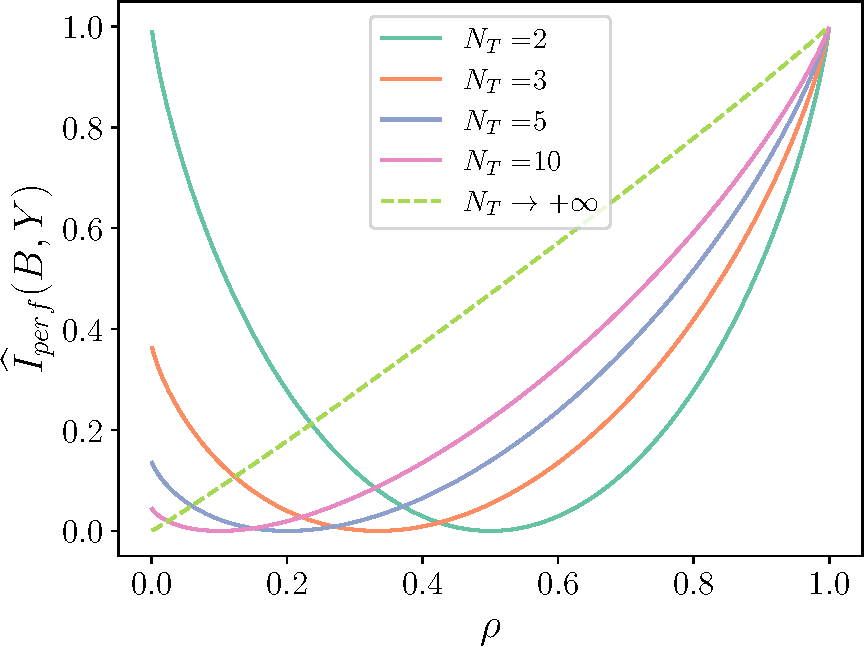
\includegraphics[width=\columnwidth]{img/MI_YZ.pdf}
    \caption{Normalized mutual information in case of perfect learner. As the number of classes $N_T$ increases, the curve smoothens. For low $N_T$ and low $\rho$ values, the anti-correlation phenomenon rises, and the mutual information increases.}
    \label{fig:MI_YZ}
\end{figure}
As it is possible to observe in Fig.~\ref{fig:MI_YZ}, a clear dependency between $\rho$ and \eqref{eq:MI_perfect} exists. In this case, the biased features and the target ones are in perfect overlap. Nonetheless, in the more general case the trained model is not a perfect learner, having $H(Y|T) \neq 0$.
The model, in this case, does not correctly classify the target for two reasons:
\begin{enumerate}
	\item It gets confused by the bias features, and it tends to learn to classify samples based on them. We model this tendency of learning biased features with $\phi$, which we call \emph{biasness}. The higher the biasness of is, the more the model relies on features which we desire to suppress, inducing bias in the model and for instance error in the model.
	\item Some extra error $\varepsilon$, non directly related to the bias features, which can be caused, for example, from stochastic unbiased effects, to underfit, or to other high-order dependencies between data. %
\end{enumerate}
We can write the discrete joint probability for $T, B, Y$, composed of the following terms.
\begin{itemize}
    \item When target, bias and prediction are aligned, the bias is aligned with the target class and correctly classified. Considering that we have not a prefect learner, we introduce the error term $\varepsilon$.
    \item When target and bias are align as well as bias and output, and the prediction is incorrect, it means that the model has not learned the correct feature and the bias is being contrasted.
    \item When target and bias are not aligned, but the prediction is correct and bias and output are aligned, it means that the model has learned the bias, introducing the error we target to minimize in this work.
    \item In all the other cases, the error of the model is due to higher-order dependencies, not directly related to the biasness $\phi$.
\end{itemize}
More formally, we can express the joint probability as:
\begin{align}
	P(T&,B,Y) = \frac{1}{N_T} \cdot \left[\delta_{tby} \rho (1 - \varepsilon) + \bar{\delta}_{ty}\delta_{tb}\delta_{by} \frac{(1-\phi)(1-\rho)}{N_T-1} \nonumber \right .\nonumber \\[1em]
	&+ \bar{\delta}_{tb}\delta_{ty}\delta_{by}\frac{\phi(1-\rho)}{N_T-1} + \delta_{tb}\bar{\delta}_{ty}\bar{\delta}_{by} \frac{\varepsilon \rho^2}{N_T-2+\rho} \nonumber \\[1em]
	&\left . + \bar{\delta}_{tb}\bar{\delta}_{ty}\bar{\delta}_{by} \frac{\varepsilon \rho (1-\rho)}{(N_T-1)(N_T-2+\rho)} \right]
    \label{eq:Pjointtotal}
\end{align}
where $\delta$ is the Kronecker delta function\footnote{for easiness of notation we suppress the index $i$: with $\delta_{tby}$ we implicitly intend that bias target and output are aligned to some $i$; hence $\delta_{ti}\delta_{bi}\delta_{yi}$}, $\bar{\delta}=1-\delta$ and $\phi,\varepsilon\in[0; 1]$.\footnote{not all the possible combinations are present in the joint probability \eqref{eq:Pjointtotal}: the missing combinations are  considered impossible, like having bias disaligned from the output but target aligned with the bias and with the output of the model (it would correspond to the case $\bar{\delta}_{by}\delta_{ty}\delta_{tb})$} We marginalize \eqref{eq:Pjointtotal} over $T$, obtaining
\begin{align}
	P(&B,Y) = \frac{1}{N_T} \cdot \left\{\delta_{by} [\rho (1 - \varepsilon) + \phi(1-\rho)] \right .\nonumber\\
	&\left .+ \bar{\delta}_{by}\left [\frac{(1-\phi)(1-\rho)}{N_T-1} + \frac{\rho\varepsilon}{N_T-2+\rho}\right ]\right\}
	\label{eq:joint_bz}
\end{align}
from which we compute the normalized mutual information
\begin{align}
    &\widehat{I}(B, Y) = \log_{N_T}\left[\rho (1 - \varepsilon) + \phi(1-\rho)\right]^{\rho (1 - \varepsilon)+ \phi(1-\rho)}\nonumber\\
    &+ \log_{N_T} \left [\frac{(1-\phi)(1-\rho)}{N_T-1} + \frac{\rho\varepsilon}{N_T-2+\rho}\right ]^{(1-\phi)(1-\rho) + \frac{(N_T-1)\rho\varepsilon}{N_T-2+\rho}}\nonumber\\
    &+ 1 + \rho\varepsilon \left(\frac{N_T-1}{N_T-2-\rho} -1 \right)\label{eq:MIcool}
\end{align}
\begin{figure}
    \centering
    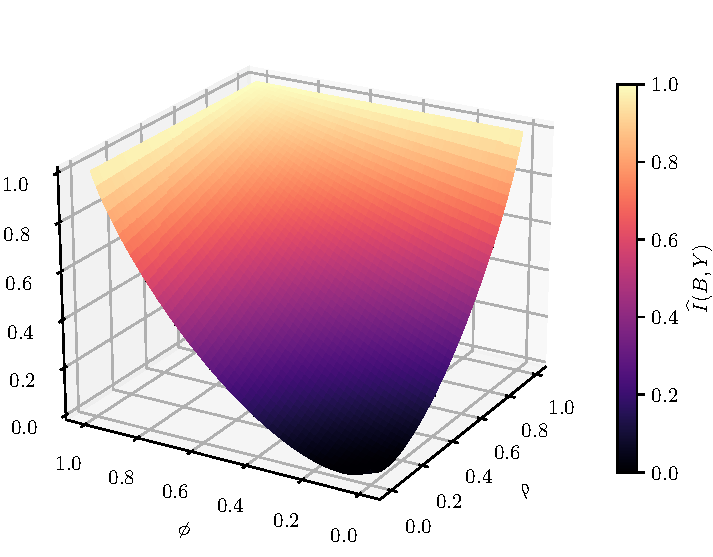
\includegraphics[width=1.0\columnwidth,trim={0 0 0 30},clip]{img/MI_YZ_full.pdf}
    \caption{Normalized mutual information between B and Y, in the case $\varepsilon=0$ and $N_T=10$. In light black, on top of the graph, level curves are drawn. In high $\rho$ regions, the mutual information is high regardless the bias tendency $\phi$ value, motivating the difficulty in learning the disentangling from biased features. A projection to a lower $\rho$ makes the problem of minimizing $\phi$ can drive the disentangling.}
    \label{fig:MI_YZ}
\end{figure}
The complete derivation can be found in the supplementary material %
and the plot for \eqref{eq:MIcool} in the case $\varepsilon=0$ is displayed in Figure~\ref{fig:MI_YZ}. 
Interestingly, we observe that for high values of $\rho$, the mutual information between the features
learned by the model and the bias is high, independently from the biasness $\phi$.
Typical learning scenarios, indeed, work in this region, where it is extremely challenging to optimize over $\phi$. On the contrary, with a lower $\rho$, the effect of $\phi$ appears evident. Towards this end, relying on a (relatively small) balanced validation set (hence, with low $\rho$) is extremely important in order to enhance the lowering of $\phi$. Directly optimizing over $\phi$ is in general not a duable strategy as the mutual information between B and Z in the typical training scenarios is very high; hence while bias removal can succeed, it will be extremely difficult to disentangle the biased features from the unbiased ones, without harming the performance.









